\section{Struktura projektu}
\subsection{Wykorzystanie języka}
Aplikacja PocztaExpress została zaprojektowana przy użyciu języka programowania C\# w oparciu o platformę .NET 8.0. Interfejs użytkownika zbudowano w technologii Windows Forms, co zapewnia wygodną obsługę i prostotę w nawigacji. 
\subsection{Wymagania sprzętowe}
Minimalne wymagania sprzętowe dla aplikacji obejmują komputer wyposażony w procesor Intel Core i3 lub jego odpowiednik od AMD. Zalecana ilość pamięci RAM to co najmniej 4 GB, aby zapewnić płynną pracę programu. Aplikacja wymaga także co najmniej 40 MB wolnego miejsca na dysku twardym w celu przechowywania plików
\subsection{Baza danych}
Aplikacja korzysta z relacyjnej bazy danych SQL Server, w której przechowywane są wszystkie dane dotyczące użytkowników i przesyłek. Baza danych zawiera dwie główne tabele. Pierwszą z nich jest tabela users, która przechowuje informacje o użytkownikach, takie jak identyfikator, imię, nazwisko, adres e-mail, hasło. Drugą kluczową tabelą jest historia\verb|_|wysylek, która rejestruje wszystkie informacje dotyczące nadanych paczek. Każda przesyłka ma przypisany unikalny identyfikator. Następną tabelą jest cennik, który przechowuje aktualne ceny kosztów nadania przesyłki. Kolejną jest tabela punkty która przechowuje punkty użytkownika. Następną są komentarze przechowujące informacje od różnych użytkowników. Zarządzanie danymi odbywa się poprzez bezpośrednie zapytania SQL wykonywane przez kod aplikacji. Używane są instrukcje SELECT do pobierania informacji o przesyłkach i użytkownikach, INSERT do dodawania nowych rekordów
\subsection{Diagram Klas}
Na rysunku 1 został przedstawiony diagram klas
\begin{figure}[!ht]
\centering
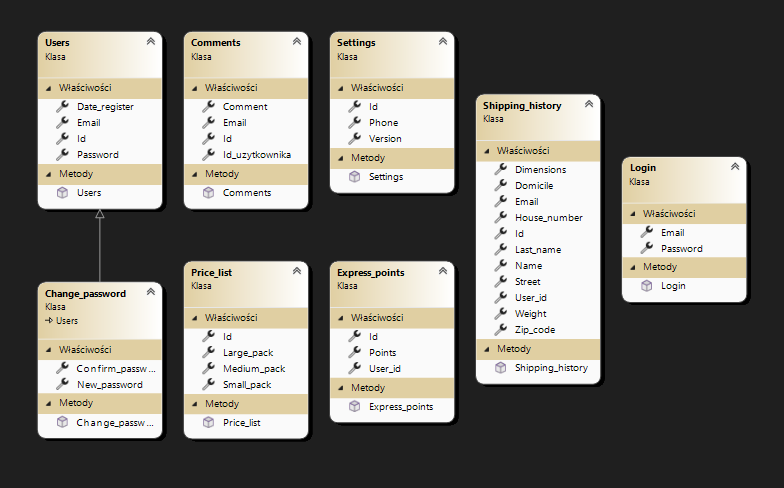
\includegraphics[width=17cm, height=8cm]{figures/diagram.png}
\caption{\footnotesize Diagram reprezentujacy klasy. }
\label{fig:plotend}
\end{figure}
\newpage
\subsection{Opis klas}
\begin{itemize}
\item \textit{Change\textunderscore password} – klasa odpowiedzialna za zmianę hasła z aktualnego na nowe
\item \textit{Comments} – klasa reprezentująca komentarze napisane przez użytkowników aplikacji (małe forum)
\item \textit{Express\textunderscore points} – klasa reprezentująca punkty za nadanie paczek
\item Login – Klasa służąca za zalogowanie się do aplikacji
\item Price\verb|_|list – Klasa odpowiedzialna za wyświetlanie aktualnych cen nadania paczki w zależności od rozmiaru paczki
\item Settings – Klasa reprezentująca ustawienia dla administratora aplikacji
\item Shipping\verb|_|history – Klasa odpowiedzialna za wyświetlenie informacji o przesyłkach już nadanych
\item Users – Klasa przechowująca listę użytkowników
\end{itemize}
